The constantly growing amounts of data and an emerging trend of incorporating unstructured  data into analytics is bringing new challenges to Business Intelligence (BI). Traditional BI solutions fall short in different aspects. Firstly, they focus only on structured data and disregard the increasing amount of information hidden in unstructured data. Secondly, they focus solely on quantitative analysis of the data: qualitative aspects, like structural dependencies in the data, are neglected. 

In the EU funded research project CUBIST, which ran from October 2010 to September 2013, those two drawbacks have ben addressed. CUBIST's approach was to complement traditional BI solutions. The CUBIST project developed methodologies and a platform that combines essential features of Semantic Technologies and BI. The most-prominent deviations from traditional BI-platforms are:
\begin{itemize}
\item The data persistency layer in the CUBIST-prototype based on a BI enabled triple store, thus CUBIST enables a user to perform BI operations over semantic data.
\item  In addition to some traditional charts, CUBIST provides novel graph-based visualizations to analyse the data.  As mathematical foundation for meaningfully clustering the data, Formal Concept Analysis is used.
\end{itemize}

From a user's perspective, CUBIST provides three different means to access the data:
\begin{itemize}
\item Factual search: First of all, using a semantic search allows the user to specifically the query the data, in order to retrieve small or large sets of entities which satisfying user-defined constraints. 
\item Explorative search: A graph-based view allows the user to interactively explore the data.
\item Visual analytics: Clusters and aggregations of data can be visually analyzed using traditional charts or novel visualizations. The selection of the visualized data as well as the visualizations are highly interactive, thus CUBIST provides ``BI as a self-service'".
\end{itemize}

A first, general diagram which depict the differences between traditional BI and CIBUST is depicted below in Figure \ref{fig:classical_v_semantic}.

CUBIST was the joint effort of seven partners, namely the project coordinator SAP SE (SAP AG during the project runtime, SAP, Germany), Ontotext (ONTO, Bulgaria), Sheffield Hallam University (SHU, UK), Centrale Rechereche S.A. (CRSA, France), Heriot-Watt University (HWU, UK), Space Applications Services (SAS, Belgium), Innovantage (INN, UK). 

SAP, ONTO, SHU and CRSA served as technological partners. During the project, they have developed a web-based prototype with the following capabilities: 
\begin{itemize}
\item Unstructured and structured data is federated in a triple store.
\item The prototype supports different information needs, i.e. searching for data, exploring and navigating in the data, and analysing the data.
\item The prototype supports ``BI as a selfservice" via comprehensive filter mechanisms and leveraging the semantics of the data.
\item The Visual Analytics of CUBIST consists of an extensive set of novel and highly interactive diagrams which allow both the quantitative and qualitative analysis of the data.
\end{itemize}

Use cases have been provided by the use case partners HWU, SAS, and INN. They have provided requirements and data sets at the beginning and constant feedback during the project lifespan, until they have finally evaluated the prototype at the project end. In CUBIST, HWU explored the semantic representation of biomedical data from a biomedical atlas and a gene expression database. SAS investigated telemetry data of a specific research device in space they monitor in mission control rooms. Finally, INN provided a job market use case which combined information from job advertisements crawled by CUBIST and an existing firmographic database.

This paper describes the approach of CUBIST, the prototype which has been developed, and the results of the project; particularly the evaluation in detail. The project as such, particularly its setup, the use cases, core technologies, and key theses are provided in section XXX. The prototype is described both in terms of technology and architecture as well as in terms of capabilities is described in section XXX: The results oft he project, particularly the results of the evaluation, are described in Section XXX. 

\begin{figure}[htbp]
   \centering
   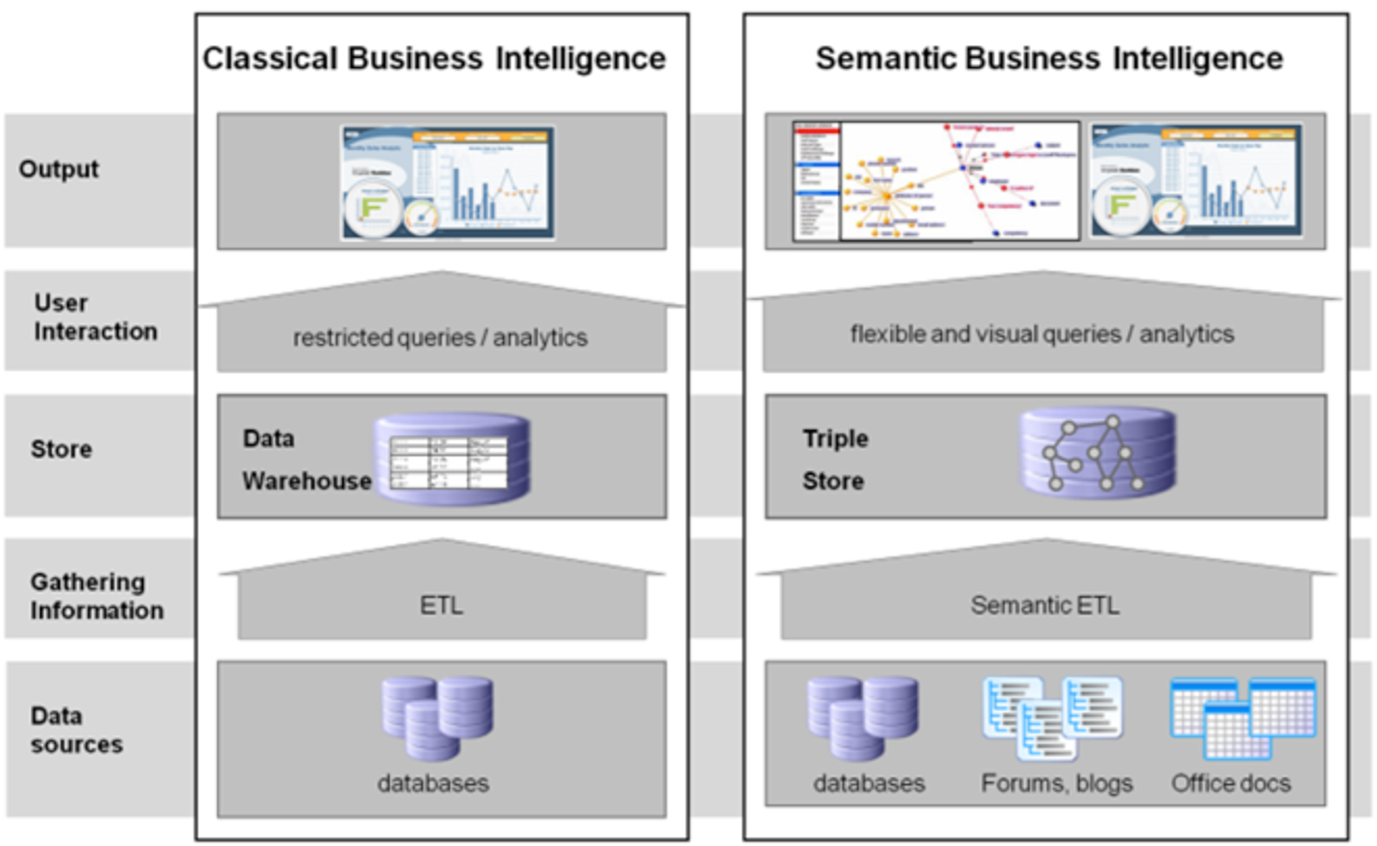
\includegraphics[width=8cm]{images/classicBI_vs_semanticBI} % requires the graphicx package
   \caption{Infographic comparing classical Business Intelligence approach against Semantic Business Intelligence.}
   \label{fig:classical_v_semantic}
\end{figure}